\scanpage{135}
U N I V E R S I T E\\
DES SCIENCES ET TECHNIQUES\\
DU LANGUEDOC\\
\rule{3cm}{0.4pt}
\hfill MONTPELLIER, le 5 Juillet 1979

Service de la Scolarité\\
MR/MB\\
\uline{Diffusion} : Liste A\\
N$^{\mathrm{o}}$3963

\begin{center}
\uline{AVIS DE SOUTENANCE D'UNE THESE DE DOCTORAT DE 3ème CYCLE} :

\uline{SCIENCES DE L'EAU}
\end{center}

\uline{NOM et Prénom du candidat} : Monsieur VELARD Frank

\uline{Titre de la thèse} : Modèles simples de comportement d'une source d'eau chaude.\\
Essai d'application aux sources thermales de la haute vallée de la Têt (Pyrénées-\\
Orientales).

\uline{Date, heure et lieu de soutenance prévus} : Mercredi 11 Juillet 1979 à 16 h.\\
\hspace*{6cm}Salle de cours N$^{\mathrm{o}}$ 10.

\uline{Nom du Directeur de la thèse} : Monsieur C. DROGUE.

\uline{Désignation du laboratoire où la thèse est préparée} : Laboratoire d'Hydrogéologie\\
et centre d'informatique géologique de l'école nationale supérieure des mines de\\
Paris à \unsure{Fontainebleau|Fôntainebleau}.

\uline{Analyse de l'ouvrage}$^{\mathrm{o}}$ :\\
Ce \unsure{travail|trabail} est un essai de représentation du fonc-\\
tionnement d'une source thermale à l'aide \unsure{d'unemodèle|d'un modèle} numérique traitant de l'écou-\\
lement ascendant dans une fente. Ce modèle est ensuite appliqué aux sources thermales\\
de la haute vallée de la Têt (\unsure{Pyénées|Pyrénées} Orientales), compte tenu des caractères géologi-\\
ques, hydrauliques et physico-chimiques de ces sources.

\uline{Durée approximative des recherches ayant abouti à la thèse} : 2 ans.

\begin{tabular}{ll}
\uline{Composition du jury proposé} : & MM. F. PROUST\\
& J. AUROUZE\\
& \unsure{C.|G.} DROGUE\\
& M. COMBARNOUS\\
& E. LEDOUX\\
& G. VASSEUR.
\end{tabular}

\begin{flushright}
Le Secrétaire Général,

\unsure{E. Siau}
\figure{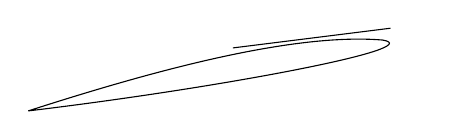
\begin{tikzpicture}[x=1cm,y=1cm]\draw (0,0) .. controls (1.4,.45) and (3.3,1.0) .. (4.5,.9) .. controls (5.1,.8) and (2.5,.3) .. (0,0);\draw (2.6,.8)--(4.6,1.05);\end{tikzpicture}}
\uline{E. SIAU}
\end{flushright}
\margin{135}
